\newpage
\subsection{Caso d'uso UC2: Registrazione}
\label{UC2}
\begin{figure}
	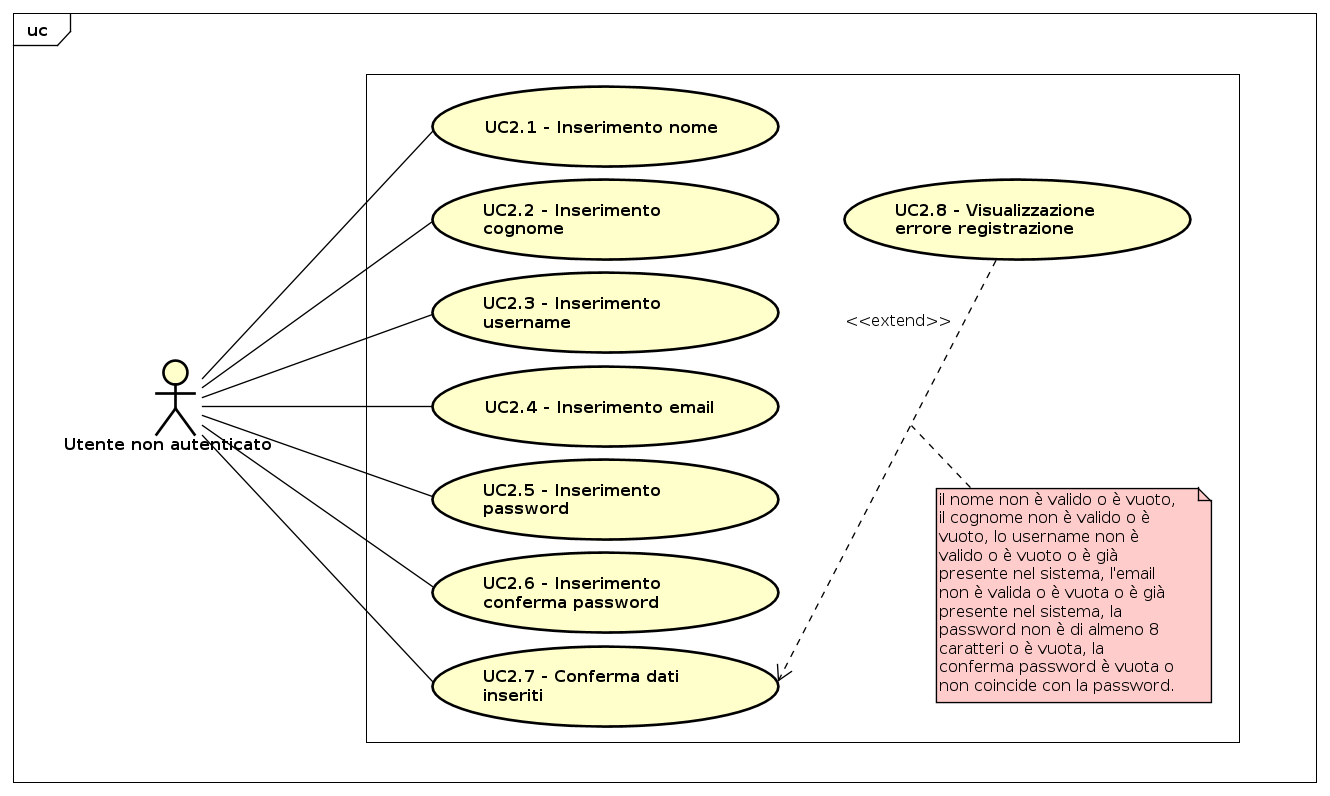
\includegraphics[scale=0.45]{UML/UC2.png}
	\caption{UC2: Registrazione}
\end{figure}
\begin{itemize}
\item \textbf{Attori}: utente non autenticato;
\item \textbf{Descrizione}: per poter usufruire dei servizi forniti dalla piattaforma, l'attore deve registrarsi inserendo email e password;
\item \textbf{Precondizione}: il sistema è avviato e mostra la pagina iniziale;
\item \textbf{Postcondizione}: il sistema ha registrato l'attore;
\item \textbf{Scenario principale}:
	\begin{enumerate}
	\item L'attore può inserire il proprio nome (UC2.1);
	\item L'attore può inserire il proprio cognome (UC2.2);
	\item L'attore può scegliere un username (UC2.3);
	\item L'attore può inserire un indirizzo e-mail (UC2.4);
	\item L'attore può inserire una password (UC2.5);
	\item L'attore può inserire una seconda volta la password (UC2.6);
	\item L'attore può confermare i dati inseriti (UC2.7).
	\end{enumerate}
\item \textbf{Estensioni}: l'attore visualizza un messaggio d'errore sulla registrazione (UC2.8);
\end{itemize}

\subsubsection{Caso d'uso UC2.1: Inserimento nome}
\begin{itemize}
\item \textbf{Attori}: utente non autenticato;
\item \textbf{Descrizione}: l'attore può inserire il proprio nome per potersi registrare;
\item \textbf{Precondizione}: il sistema visualizza l'area per effettuare la registrazione;
\item \textbf{Postcondizione}: l'attore ha inserito il nome;
\item \textbf{Scenario principale}: l'attore inserisce il proprio nome per potersi registrare.
\end{itemize}

\subsubsection{Caso d'uso UC2.2: Inserimento cognome}
\begin{itemize}
\item \textbf{Attori}: utente non autenticato;
\item \textbf{Descrizione}: l'attore può inserire il proprio cognome per potersi registrare;
\item \textbf{Precondizione}: il sistema visualizza l'area per effettuare la registrazione;
\item \textbf{Postcondizione}: l'attore ha inserito il cognome;
\item \textbf{Scenario principale}: l'attore inserisce il proprio cognome per potersi registrare.
\end{itemize}

\subsubsection{Caso d'uso UC2.3: Inserimento username}
\begin{itemize}
\item \textbf{Attori}: utente non autenticato;
\item \textbf{Descrizione}: l'attore può inserire il proprio username per potersi registrare;
\item \textbf{Precondizione}: il sistema visualizza l'area per effettuare la registrazione;
\item \textbf{Postcondizione}: l'attore ha inserito lo username;
\item \textbf{Scenario principale}: l'attore inserisce il proprio username per potersi registrare.
\end{itemize}

\subsubsection{Caso d'uso UC2.4: Inserimento e-mail}
\begin{itemize}
\item \textbf{Attori}: utente non autenticato;
\item \textbf{Descrizione}: l'attore può inserire il proprio indirizzo e-mail per potersi registrare;
\item \textbf{Precondizione}: il sistema visualizza l'area per effettuare la registrazione;
\item \textbf{Postcondizione}: l'attore ha inserito l'e-mail;
\item \textbf{Scenario principale}: l'attore inserisce il proprio indirizzo e-mail per potersi registrare.
\end{itemize}

\subsubsection{Caso d'uso UC2.5: Inserimento password}
\begin{itemize}
\item \textbf{Attori}: utente non autenticato;
\item \textbf{Descrizione}: l'attore può inserire una password per potersi registrare;
\item \textbf{Precondizione}: il sistema visualizza l'area per effettuare la registrazione;
\item \textbf{Postcondizione}: l'attore ha inserito la password;
\item \textbf{Scenario principale}: l'attore inserisce una password per potersi registrare.
\end{itemize}

\subsubsection{Caso d'uso UC2.6: Inserimento conferma password}
\begin{itemize}
\item \textbf{Attori}: utente non autenticato;
\item \textbf{Descrizione}: l'attore può inserire nuovamente la password scelta;
\item \textbf{Precondizione}: il sistema visualizza l'area per effettuare la registrazione;
\item \textbf{Postcondizione}: l'attore ha inserito la conferma della password;
\item \textbf{Scenario principale}: l'attore inserisce nuovamente la password scelta.
\end{itemize}

\subsubsection{Caso d'uso UC2.7: Conferma registrazione}
\begin{itemize}
\item \textbf{Attori}: utente non autenticato;
\item \textbf{Descrizione}: l'attore può confermare i dati inseriti;
\item \textbf{Precondizione}: il sistema visualizza l'area per effettuare la registrazione;
\item \textbf{Postcondizione}: il sistema ha ricevuto i dati per la registrazione;
\item \textbf{Scenario principale}: l'attore conferma i dati inseriti.
\end{itemize}

\subsubsection{Caso d'uso UC2.8: Visualizzazione errore registrazione}
\begin{itemize}
\item \textbf{Attori}: utente non autenticato;
\item \textbf{Descrizione}: l'attore può visualizzare un messaggio d'errore nel caso si fossero verificati uno o più scenari alternativi durante la fase di registrazione;
\item \textbf{Precondizione}: il sistema ha ricevuto dei dati errati per la registrazione;
\item \textbf{Postcondizione}: il sistema avvisa l'attore dell'errore verificatosi tramite un opportuno messaggio;
\item \textbf{Scenario principale}: l'attore visualizza un messaggio d'errore.
\end{itemize}
